
\documentclass[12pt,aspectratio=169]{beamer}

\input{style.tex}

\begin{document}

{\usebackgroundtemplate{\tikz\node[opacity=0.4,inner sep=0]{
\includegraphics[width=\paperwidth,height=\paperheight]{images/header}};}%
\begin{frame}[plain]
	\vspace{0.5cm}
	\title{\large \begin{spacing}{1.0}Fondamenti di Machine Learning\end{spacing}\vspace{0.25em}
		\normalsize \begin{spacing}{1.0}\textbf{Laurea Triennale in Ingegneria delle Comunicazioni}\end{spacing}\vspace{0.5em}}
	\subtitle{\Large \textbf{4: $k$-nearest neighbors ed overfitting}}
	\date{
		{
\includegraphics[scale=0.8]{images/Uniroma1}}
	}
	\author{
		\setlength{\tabcolsep}{2pt}
		\begin{tabular}{rl}
			\textbf{Lecturer}: & S. Scardapane \\
		\end{tabular}
	}\titlepage
\end{frame}
}

\part{1}

\section{Instance-based learning}
\subsection{$k$-nearest neighbors}

\begin{frame}{Modelli locali e globali}

	Nel caso del LS costruiamo un modello \textit{globale} per tutto lo spazio $\mathbb{R}^d$. Quindi, modificare anche un singolo esempio di training (es., aggiungendo un \myalert{outlier}) influenza tutte le predizioni.

	In un modello \textit{locale}, invece, le predizioni sono influenzate solo dai punti di training ad esso vicine (\myalert{instance-based learning}).

	Qui di seguito vediamo l'implementazione più semplice di questa idea, chiamata $k$-Nearest Neighbours ($k$-NN), che predice la media (o la mediana) dei $k$ punti più simili.

\end{frame}

\begin{frame}{Definizione del $k$-NN}

	Denotiamo con $\mathcal{N}_k(\mathbf{x})$ l'insieme degli indici dei $k$ punti più simili ad $\mathbf{x}$ nel training set $\mathcal{S}$, ad esempio con la distanza Euclidea:
	%
	\begin{equation}
		d(\mathbf{x}, \mathbf{z}) = \sqrt{\sum_i (x_i-z_i)^2} \,.
	\end{equation}
	%
	Dato un punto $\mathbf{x}$, per un problema di regressione il $k$-NN predice la media calcolata in $\mathcal{N}_k(\mathbf{x})$:
	%
	\begin{equation}
		f(\mathbf{x}) = \frac{1}{k}\sum_{i \in \mathcal{N}_k(\mathbf{x})} y_i
	\end{equation}

\end{frame}

\begin{frame}{$k$-NN per la classificazione}

	In un problema di \myalert{classificazione}, a differenza della regressione, le etichette $y_i$ appartengono ad un insieme discreto e finito di categorie (es., ``spam'' o ``non spam'').

	Per adattare il $k$-NN alla classificazione, il modello predice la classe più frequente tramite un \myalert{voto di maggioranza} tra i $k$ punti contenuti in $\mathcal{N}_k(\mathbf{x})$:
	%
	\begin{equation}
		f(\mathbf{x}) = \arg\max_{c} \sum_{i \in \mathcal{N}_k(\mathbf{x})} I(y_i = c)
	\end{equation}
	%
	dove $I(\cdot)$ vale $1$ se l'argomento è vero, $0$ altrimenti. In caso di parità, il pareggio può essere risolto arbitrariamente (es., casualmente).

\end{frame}

\begin{frame}{Considerazioni sul $k$-NN}

	Nel $k$-NN non è necessario allenare nulla, ma in fase di predizione è necessario avere l'intero training set in memoria, ed una procedura efficiente per calcolare i $k$ valori più vicini. Questo può essere sconveniente per dataset molto grandi.

	Il $k$-NN viene anche detto un modello \myalert{non parametrico}, nel senso che la sua complessità varia al variare del numero dei punti (intuitivamente, ogni esempio aggiunto al training set rende la decision boundary leggermente più complessa).

\end{frame}

\begin{whiteframe}{Esempio - $1$-NN}

	\begin{figure}
		\centering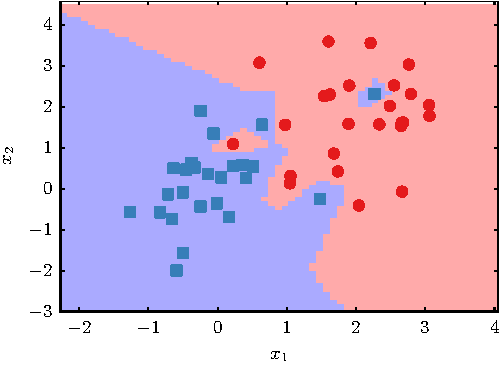
\includegraphics{../scripts/1nn.pdf}
		\caption{Decision boundary del $k$-NN con $k=1$.}
	\end{figure}

\end{whiteframe}

\begin{whiteframe}{Esempio - $10$-NN}

	\begin{figure}
		\centering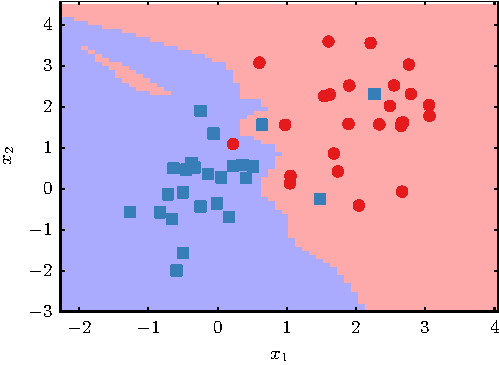
\includegraphics{../scripts/1nn-2.pdf}
		\caption{Decision boundary del $k$-NN con $k=10$.}
	\end{figure}

\end{whiteframe}

\begin{whiteframe}{Esempio - $25$-NN}

	\begin{figure}
		\centering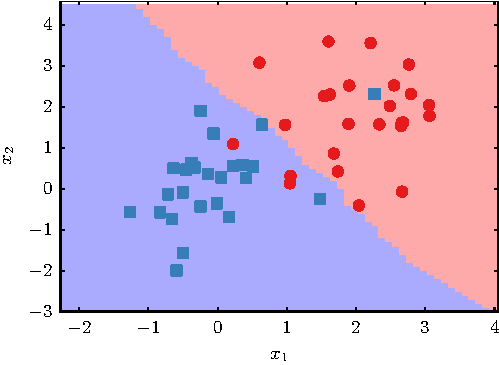
\includegraphics{../scripts/1nn-3.pdf}
		\caption{Decision boundary del $k$-NN con $k=25$.}
	\end{figure}

\end{whiteframe}

\begin{frame}{Weighted $k$-NN}

	Possiamo generalizzare il $k$-NN supponendo di pesare diversamente i contributi da punti vicini o lontani:

	$$
		f(\vc{x}) = \sum_{i \in \mathcal{N}_k(\vc{x})} s_i y_i \,\, \text{ con } s_i = \frac{s(\mathbf{x}, \mathbf{x}_i)}{\sum_{j \in \mathcal{N}_k(\vc{x})} s(\mathbf{x}, \mathbf{x}_j)} \,.
	$$

	dove $s(\mathbf{x}, \mathbf{x}_i) \propto 1/d(\mathbf{x}, \mathbf{x}_i)$ è una qualunque misura di \alert{similarità} (inverso della distanza).

\end{frame}

\begin{whiteframe}{Weighted $k$-NN vs. uniform $k$-NN}

	\begin{figure}
		\centering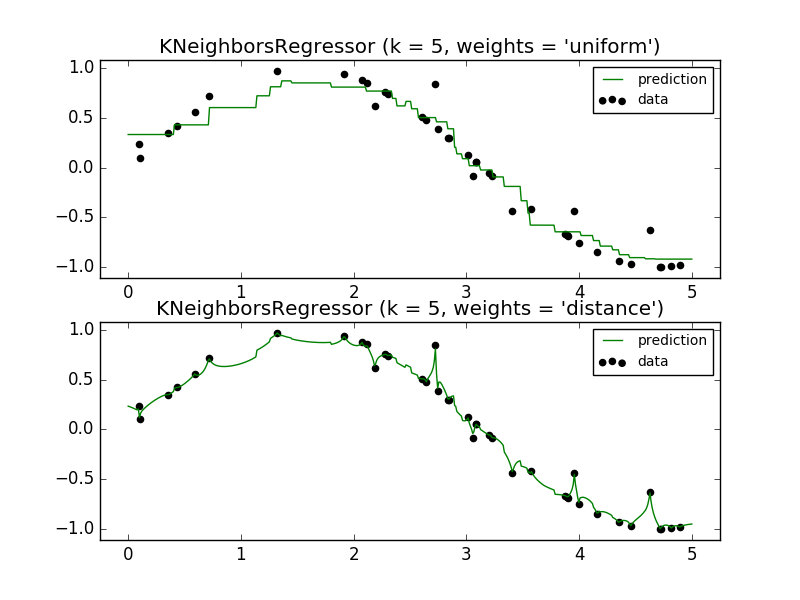
\includegraphics[width=9cm,keepaspectratio]{./images/sphx_glr_plot_regression_0011.png} %
		\vspace{-1em}\caption{Image source: \href{http://scikit-learn.org/stable/modules/neighbors.html}{Nearest neighbors in scikit-learn}}
	\end{figure}

\end{whiteframe}

\begin{frame}{Manhattan distance}

	In alternativa alla distanza Euclidea possiamo considerare la cosiddetta distanza di \textbf{Manhattan} (o \textbf{taxicab}):
	%
	$$
		d(\vc{x}, \vc{z}) = \sum_{i=1}^d \lvert x_{i} - z_{i} \rvert \,.
	$$
	%
	I parametri di configurazione di un algoritmo (es., $k$ nel $k$-NN, la funzione di distanza da usare, il learning rate) vengono detti gli \myalert{iper-parametri} del modello. Vedremo più avanti tecniche per la loro selezione.

\end{frame}

\begin{whiteframe}{Visualizzazione della distanza di Manhattan}

	\begin{figure}
		\centering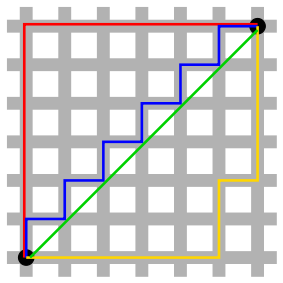
\includegraphics[width=5cm]{./images/283px-Manhattan_distance.png}
		\caption{Visualizzazione della distanza di Manhattan [Wikipedia].}
	\end{figure}

\end{whiteframe}

\section{Topic aggiuntivi}

\subsection{Overfitting e complessità}

\begin{frame}{Misure di performance}

	Come già accennato, un modo di valutare le performance di un modello è tenere un dataset indipendente di valutazione (\myalert{holdout method}):
	%
	\begin{itemize}
		\item Un \textbf{training set} per scegliere i parametri del nostro modello.
		\item Un \textbf{test set} (indipendente) per valutarne l'errore.
	\end{itemize}
	%
	Vedremo più avanti tecniche (e metriche) più sofisticate per valutare gli algoritmi di apprendimento. In un problema di classificazione, se la proporzione di classi è mantenuta in entrambi i dataset, parliamo di \myalert{holdout stratificato}.

\end{frame}

\begin{frame}{Underfitting ed overfitting}

	Per definizione, $1$-NN ha sempre \textit{zero} errore sul dataset di training. Le sue performance sul dataset di test sono però nettamente inferiori: in questo caso parliamo di \myalert{overfitting}.

	All'opposto, il $25$-NN ha errori su training e test simili, ma superiori a quelli del $10$-NN. In questo caso parliamo invece di \myalert{underfitting} dell'algoritmo.

	In generale, l'apprendimento supervisionato è molto diverso dalla pura \textit{memorizzazione} degli esempi di training, in quanto ci interessa estrapolare (generalizzare) su dati futuri.

\end{frame}

\begin{frame}{Complessità ed iperparametri}

	Il parametro $k$ nel $k$-NN determina la \myalert{complessità} del modello: variandolo, possiamo passare da un modello molto semplice (costante su tutto il dataset) ad un dataset altamente non-lineare. In molti casi, l'overfitting dipende dalla scelta di una complessità troppo alta rispetto al dataset.

	Più in generale, qualsiasi parametro che può essere scelto dall'utente (e non dalla procedura di apprendimento) viene detto un \myalert{iper-parametro}. La scelta degli iper-parametri ottimi per un problema è detto \myalert{model selection}.

\end{frame}

\begin{frame}{Visualizzazione dell'overfitting}

	\begin{figure}
		\centering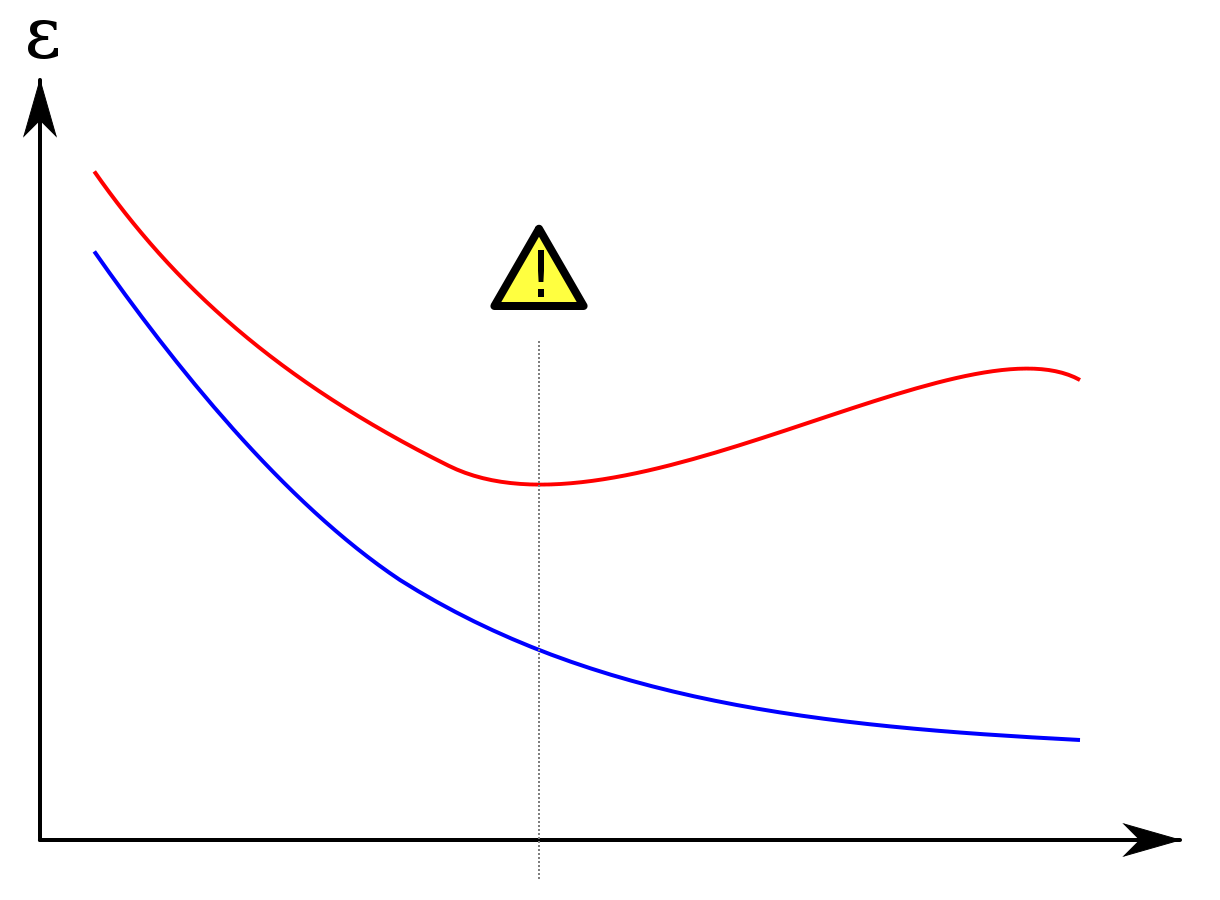
\includegraphics[width=8cm]{./images/1220px-Overfitting_svg.png}
		\caption{Da Wikipedia: errore (asse $y$) vs. una misura di complessità (asse $x$). Errore di training e test sono blu e rosso, rispettivamente.}
	\end{figure}

\end{frame}

\subsection{Bias variance decomposition}

\begin{frame}{Bias-variance decomposition}

	Diversi ragionamenti che abbiamo fatto in precedenza (es., sull'overfitting) possono essere formalizzati con la cosiddetta  \myalert{bias-variance decomposition}. La sua derivazione è leggermente più tecnica di quanto visto finora, ma richiede solo di conoscere alcune proprietà del valore atteso:
	%
	\begin{align}
		\mathbb{E}[x+y] = \mathbb{E}[x] + \mathbb{E}[y]                         &  & \texttt{Linearità}    \\
		\mathbb{E}[xy] = \mathbb{E}[x]\mathbb{E}[y] \text{ se } p(x,y)=p(x)p(y) &  & \texttt{Indipendenza}
	\end{align}

\end{frame}

\begin{frame}{Setup}

	Nel caso più semplice, assumiamo che i nostri dati siano generati come segue:
	%
	\begin{equation}
		y = g(\mathbf{x}) + \varepsilon \,,
	\end{equation}
	%
	dove $g(\cdot)$ è deterministica (ma sconosciuta), $\varepsilon \sim \mathcal{N}(0, \sigma^2)$, e quindi:
	%
	\begin{equation}
		p(y \mid \mathbf{x}) = \mathcal{N}(y; g(\mathbf{x}), \sigma^2) \,.
	\end{equation}
	%
	Cerchiamo di approssimare questo dataset con una qualche $f(\mathbf{x})$ (senza assunzioni), minimizzando la squared loss $(y - f(\mathbf{x}))^2$.

\end{frame}

\begin{frame}{Derivazione del tradeoff}

	Siamo interessati a capire come si distribuisce tale errore quadratico medio:
	%
	\begin{equation}
		\mathbb{E}[(y-f(\mathbf{x}))^2] = \mathbb{E}[y^2] + \mathbb{E}[f(\mathbf{x})^2] - 2\mathbb{E}[yf(\mathbf{x})]
	\end{equation}
	%
	dove (informalmente) il valore atteso è calcolato rispetto ad ogni possibile scelta di dataset di training. Ricordando $\text{Var}(x) = \mathbb{E}[x^2] - \mathbb{E}[x]^2$ possiamo riscrivere il secondo termine come:
	%
	\begin{equation}
		\mathbb{E}[f(\mathbf{x})^2] = \text{Var}(f(\mathbf{x})) + \mathbb{E}[f(\mathbf{x})]^2
	\end{equation}

\end{frame}

\begin{frame}{Derivazione del tradeoff (2)}

	Il primo termine può essere semplificato date le nostre assunzioni sui dati:
	%
	\begin{equation}
		\mathbb{E}[y^2] = \mathbb{E}[(g(\mathbf{x}) + \varepsilon)^2] = \mathbb{E}[g(\mathbf{x})^2] + \mathbb{E}[\varepsilon^2] + 2\mathbb{E}[\varepsilon g(\mathbf{x})]
	\end{equation}
	%
	Da cui:
	%
	\begin{align}
		\mathbb{E}[g(\mathbf{x})^2] = g(\mathbf{x})^2                                                  &  & \texttt{$g$ non dipende dal dataset}  \\
		\mathbb{E}[\varepsilon^2] = \sigma^2                                                           &  & \texttt{Definizione di una Gaussiana} \\
		2\mathbb{E}[\varepsilon g(\mathbf{x})] = 2\mathbb{E}[g(\mathbf{x})]\mathbb{E}[\varepsilon] = 0 &  & \texttt{Indipendenza}
	\end{align}

\end{frame}

\begin{frame}{Derivazione del tradeoff (3)}

	Rimane l'ultimo termine:
	%
	\begin{equation}
		2\mathbb{E}[yf(\mathbf{x})] = 2\mathbb{E}[(g(\mathbf{x}) + \varepsilon)f(\mathbf{x})] = 2\mathbb{E}[g(\mathbf{x})f(\mathbf{x})] + \underbrace{2\mathbb{E}[\varepsilon f(\mathbf{x})]}_{=0}
	\end{equation}
	%
	Ed infine, sempre per l'indipendenza delle due variabili:
	%
	\begin{equation}
		2\mathbb{E}[g(\mathbf{x})f(\mathbf{x})] = 2g(\mathbf{x})\mathbb{E}[f(\mathbf{x})]
	\end{equation}

\end{frame}

\begin{frame}{Derivazione del tradeoff (4)}

	Rimettendo tutto insieme:
	%
	\begin{equation}
		\mathbb{E}[(y-f(\mathbf{x}))^2] = \mathbb{E}[f(\mathbf{x})]^2 + g(\mathbf{x})^2 - 2g(\mathbf{x})\mathbb{E}[f(\mathbf{x})] + \text{Var}(f(\mathbf{x})) + \sigma^2
	\end{equation}
	%
	Definendo:
	%
	\begin{equation}
		\text{Bias}(f(\mathbf{x})) = \mathbb{E}[f(\mathbf{x})] - g(\mathbf{x})
	\end{equation}
	%
	Otteniamo:
	%
	\begin{equation}
		\mathbb{E}[(y-f(\mathbf{x}))^2] = \text{Bias}(f(\mathbf{x}))^2 + \text{Var}(f(\mathbf{x})) + \sigma^2
	\end{equation}

\end{frame}

\begin{frame}{Commenti}

	Vediamo che l'errore quadratico medio si decompone su tre assi:
	%
	\begin{enumerate}
		\item Il \myalert{bias} descrive l'errore medio compiuto da $f$, mediato su tutti i possibili dataset. Ad esempio, se $g(x)$ è lineare, la soluzione data dal least-squares ha bias $0$.
		\item La \myalert{varianza} descrive quanto l'errore varia per un \textit{singolo} dataset.
		\item Il \myalert{rumore} descrive la componente della loss che non può essere ridotta in quanto dipende dalla aleatorietà dei dati stessi.
	\end{enumerate}
	%
	Ritornando al $k$-NN, per $k$ piccoli abbiamo un bias basso ma una varianza molto alta, mentre per $k$ larghi abbiamo un bias molto grande ma una varianza molto piccola. Il giusto trade-off si ottiene per una scelta di $k$ che bilancia questi due fattori.

\end{frame}

\subsection{Curse of dimensionality}

\begin{frame}{La maledizione della dimensionalità}

	Finora abbiamo considerato problemi relativamente semplici, con una dimensionalità $d$ bassa. Non tutti gli algoritmi, però, scalano ugualmente bene all'aumentare della dimensionalità.

	Ad esempio, consideriamo questa semplice variante del $k$-NN: dividiamo lo spazio Euclideo in celle di dimensioni fissa; per ogni cella prendiamo tutti gli elementi del training set che vi cadono dentro; assegniamo un voto di maggioranza \textit{all'intera cella} sulla base di questi punti.

\end{frame}

\begin{whiteframe}{Visualizzazione}

	\begin{figure}
		\centering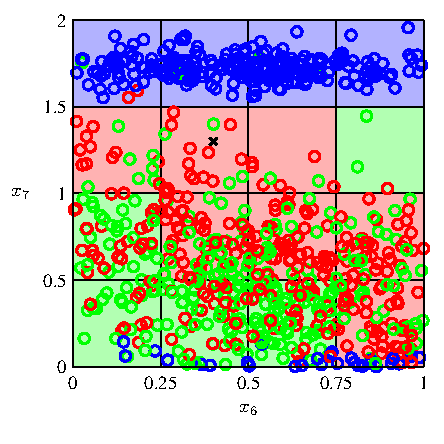
\includegraphics[scale=0.8]{./images/Figure1.20.pdf} %
		\vspace{-0.5em}\caption{Semplificazione del $k$-NN in cui scegliamo una predizione per ogni cella in cui viene ripartito lo spazio Euclideo (riprodotto da Bishop e Bishop, 2023).}
	\end{figure}

\end{whiteframe}

\begin{whiteframe}{Curse of dimensionality}

	\begin{figure}
		\centering
		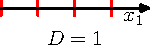
\includegraphics[width=0.2\textwidth]{images/Figure1.21a.pdf} \hspace{2em}
		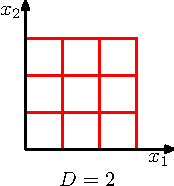
\includegraphics[width=0.2\textwidth]{images/Figure1.21b.pdf} \hspace{2em}
		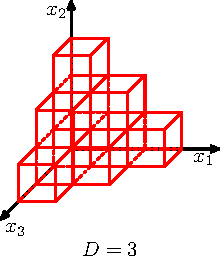
\includegraphics[width=0.2\textwidth]{images/Figure1.21c.pdf} \hfill
		\caption{Il numero di elementi necessari a riempire lo spazio mantenendo la stessa densità cresce esponenzialmente con la dimensione dello spazio (riprodotto da Bishop e Bishop, 2023).}
	\end{figure}

\end{whiteframe}

\begin{frame}{Curse of dimensionality}

	Si usa il termine \textit{curse of dimensionality} per riferirsi a tutte quelle proprietà che dipendono in maniera esponenziale dalla dimensionalità dello spazio (es., i dati necessari a campionare lo spazio nell'esempio precedente).

	Come altro esempio: in uno spazio ad $n$ dimensioni, il volume di una sfera di raggio $r$ si può scrivere come $V(r) = k_n r^n$, dove $k_n$ è una costante che dipende da $n$. La frazione di volume contenuta tra $r-\epsilon$ ed $r$ è quindi:
	%
	\begin{equation}
		\frac{V(r) - V(r-\epsilon)}{V(r)} = r - (r-\epsilon)^n
	\end{equation}
	%
	Per grandi $n$, la maggior parte del volume di una sfera è concentrato sulla superficie!

\end{frame}

\begin{whiteframe}{Volume di una sfera $n$-dimensionalità}

	\begin{figure}
		\centering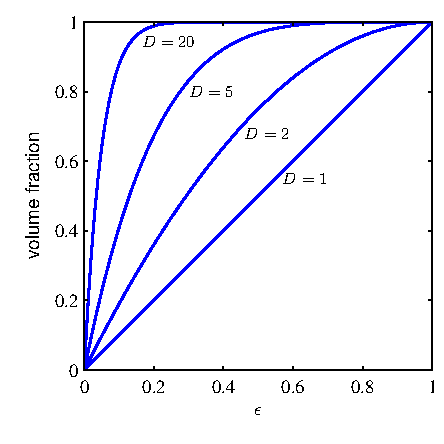
\includegraphics[scale=0.8]{./images/Figure1.22.pdf} %
		\vspace{-1em}\caption{Grafico della frazione $\frac{V(r) - V(r-\epsilon)}{V(r)}$ per vari $n$, supponendo $r=1$ (riprodotto da Bishop e Bishop, 2023).}
	\end{figure}

\end{whiteframe}

\end{document}
